\documentclass[tikz,border=2pt]{standalone}
\usepackage{amsmath}
\usetikzlibrary{arrows.meta,calc}

\begin{document}
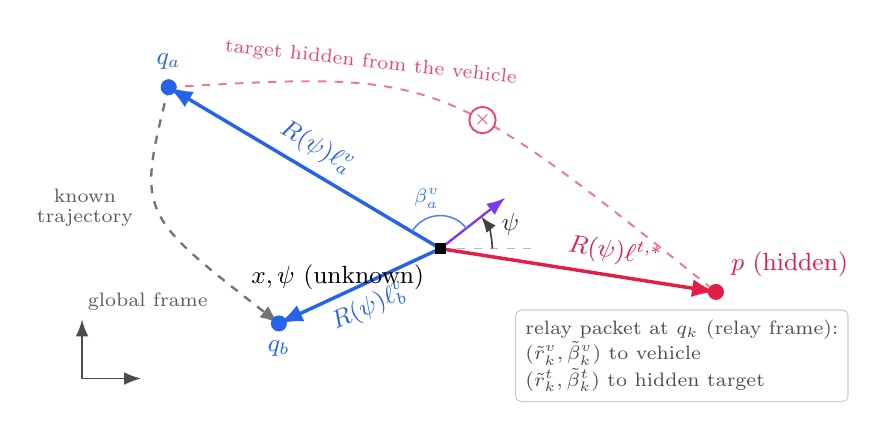
\begin{tikzpicture}[
  x=1cm,
  y=1cm,
  >=Latex,
  point/.style={circle,fill=#1,draw=#1,inner sep=1.9pt},
  packet/.style={line width=1.25pt,-Latex},
  note/.style={font=\scriptsize,text=black!65},
  every node/.style={font=\small}
]
\definecolor{figblue}{RGB}{37,99,235}
\definecolor{figred}{RGB}{225,29,72}
\definecolor{figpurple}{RGB}{124,58,237}

\coordinate (qa) at (1.55,4.15);
\coordinate (qb) at (2.95,1.15);
\coordinate (x)  at (5.00,2.10);
\coordinate (p)  at (8.50,1.55);

% Global reference frame: the one frame that is known.
\draw[-Latex, black!70, line width=0.7pt] (0.45,0.45) -- ++(0.75,0);
\draw[-Latex, black!70, line width=0.7pt] (0.45,0.45) -- ++(0,0.75);
\node[note, anchor=west] at (0.40,1.42) {global frame};

% Known vehicle motion between the two poses.
\draw[black!55, dashed, -Latex, line width=0.85pt]
  (qa) .. controls (1.15,2.55) .. (qb);
\node[note, align=center, anchor=east] at (1.22,2.62) {known\\[-1pt]trajectory};

% The vehicle never measures the target directly.
\draw[figred!60, dashed, line width=0.7pt] (qa) .. controls (5.0,4.35) .. (p)
  node[pos=0.33, above=1pt, sloped, note, text=figred!80] {target hidden from the vehicle}
  node[pos=0.6, circle, solid, draw=figred!80, fill=white, inner sep=0.5pt,
       font=\scriptsize, text=figred!80] {$\times$};

% Relay heading (unknown yaw psi, measured from the global-parallel axis).
\draw[gray!55, dashed, line width=0.55pt] (x) -- ++(1.15,0);
\draw[-Latex, figpurple, line width=0.85pt] (x) -- ++(38:1.05);
\draw[-Latex, black!75, line width=0.6pt]
  ($(x)+(0.66,0)$) arc[start angle=0, end angle=38, radius=0.66];
\node[black!80] at ($(x)+(19:0.94)$) {$\psi$};

% Measurement rays: global realizations of the relay-frame packet vectors.
\draw[packet, figblue] (x) -- node[above, sloped, text=figblue] {$R(\psi)\ell_a^v$} (qa);
\draw[packet, figblue] (x) -- node[below, sloped, text=figblue] {$R(\psi)\ell_b^v$} (qb);
\draw[packet, figred]  (x) -- node[above, sloped, text=figred, pos=0.62] {$R(\psi)\ell^{t,*}$} (p);

% Example bearing: measured from the relay heading, not the global axis.
\draw[figblue!80, line width=0.55pt]
  ($(x)+(38:0.42)$) arc[start angle=38, end angle=149, radius=0.42];
\node[font=\scriptsize, text=figblue!90] at ($(x)+(105:0.66)$) {$\beta_a^v$};

% What one relay packet actually contains.
\node[draw=black!20, rounded corners=2pt, fill=white, anchor=south west,
      align=left, font=\scriptsize, text=black!70, inner sep=3.5pt] at (5.95,0.15)
  {relay packet at $q_k$ (relay frame):\\
   $(\tilde r^v_k,\tilde\beta^v_k)$ to vehicle\\
   $(\tilde r^t_k,\tilde\beta^t_k)$ to hidden target};

\node[point=figblue, label={[text=figblue]above:$q_a$}] at (qa) {};
\node[point=figblue, label={[text=figblue]below:$q_b$}] at (qb) {};
\node[rectangle, fill=black, inner sep=2.1pt,
      label={[text=black]below left:{$x,\psi$ (unknown)}}] at (x) {};
\node[point=figred, label={[text=figred]above right:{$p$ (hidden)}}] at (p) {};
\end{tikzpicture}
\end{document}
